Hạ đường cao BH xuống đường thẳng đi qua AC. Phân giác góc $\widehat{\text{ABC}}$ cắt đoạn AC tại điểm M, phân giác góc $\widehat{\text{CBT}}$ cắt đường kéo dài đoạn AC lên phía A tại điểm N. Trung điểm của M và N là O. Ta vẽ đường tròn tâm O đi qua M và N, thế thì đường cong này cũng sẽ phải đi qua B do $\widehat{\text{MBN}}=90^o$ (xem hình minh họa \textbf{a}). 

\ \
 
Từ \textit{định lý đường phân giác}, áp dụng cho phân giác trong và phân giác ngoài của góc $\widehat{\text{ABC}}$, ta có tỉ số $\overline{\text{AB}}:\overline{\text{BC}} = s_1:s_2$ là bằng với tỉ số $\overline{\text{AM}}:\overline{\text{MC}}$ và $\overline{\text{AN}}:\overline{\text{NC}}$. Chúng ta có thể chứng minh vắn như sau: 
 \begin{itemize}
     \item Hạ đường cao AI xuống BM và CJ xuống đường kéo dài BM về phía M (xem hình minh họa \textbf{b}). Theo định lý Thalès, với AI $\parallel$ CJ, ta có $\overline{\text{AM}}:\overline{\text{MC}} = \overline{\text{AI}}:\overline{\text{CJ}}$. Từ các liên hệ lượng giác $\overline{\text{AI}}:\overline{\text{AB}}=\sin \widehat{\text{ABI}}$ và $\overline{\text{CJ}}:\overline{\text{BC}}=\sin \widehat{\text{JBC}}$, chú ý rằng $\widehat{\text{ABI}}=\widehat{\text{JBC}}$ vì BM là phân giác trong của góc $\widehat{\text{ABC}}$, nên tới đây chúng ta thu được đẳng thức $\overline{\text{AM}}:\overline{\text{MC}}=\overline{\text{AB}}:\overline{\text{BC}}=s_1:s_2$.
     \item Hạ đường cao AK xuống BN và CL xuống đường kéo dài BN về phía B (xem hình minh họa \textbf{c}). Theo định lý Thalès, với AK $\parallel$ CL, ta có $\overline{\text{AN}}:\overline{\text{NC}} = \overline{\text{AK}}:\overline{\text{CL}}$. Từ các liên hệ lượng giác $\overline{\text{AK}}:\overline{\text{AB}}=\sin \widehat{\text{ABK}}$ và $\overline{\text{LC}}:\overline{\text{BC}}=\sin \widehat{\text{LBC}}$, chú ý rằng $\widehat{\text{ABK}}=\widehat{\text{LBC}}$ vì BN là phân giác ngoài của góc $\widehat{\text{ABC}}$, nên tới đây chúng ta thu được đẳng thức $\overline{\text{AN}}:\overline{\text{NC}}=\overline{\text{AB}}:\overline{\text{BC}}=s_1:s_2$.
 \end{itemize}

 \ \ 

Biết $\overline{\text{AC}}=s_3$, ta xác định được:
\begin{equation}
\overline{\text{AM}}=\frac{s_1}{s_1+s_2}s_3 \ , \ \overline{\text{MC}}=\frac{s_2}{s_1+s_2}s_3 \ , \ \overline{\text{AN}}=\frac{s_1}{-s_1+s_2}s_3 \ , \ \overline{\text{NC}}=\frac{s_2}{-s_1+s_2}s_3 \ ,
\label{distance}
\end{equation}
và bán kính đường tròn tâm O đường kính MN:
\begin{equation}
\overline{\text{OM}} = \overline{\text{ON}} = \frac12 \overline{\text{MN}} = \frac12 \Big( \overline{\text{MA}} + \overline{\text{AN}} \Big) = \frac{s_1 s_2}{-s_1^2 + s_2^2} s_3 \ .
\label{radius}
\end{equation}

\begin{center}
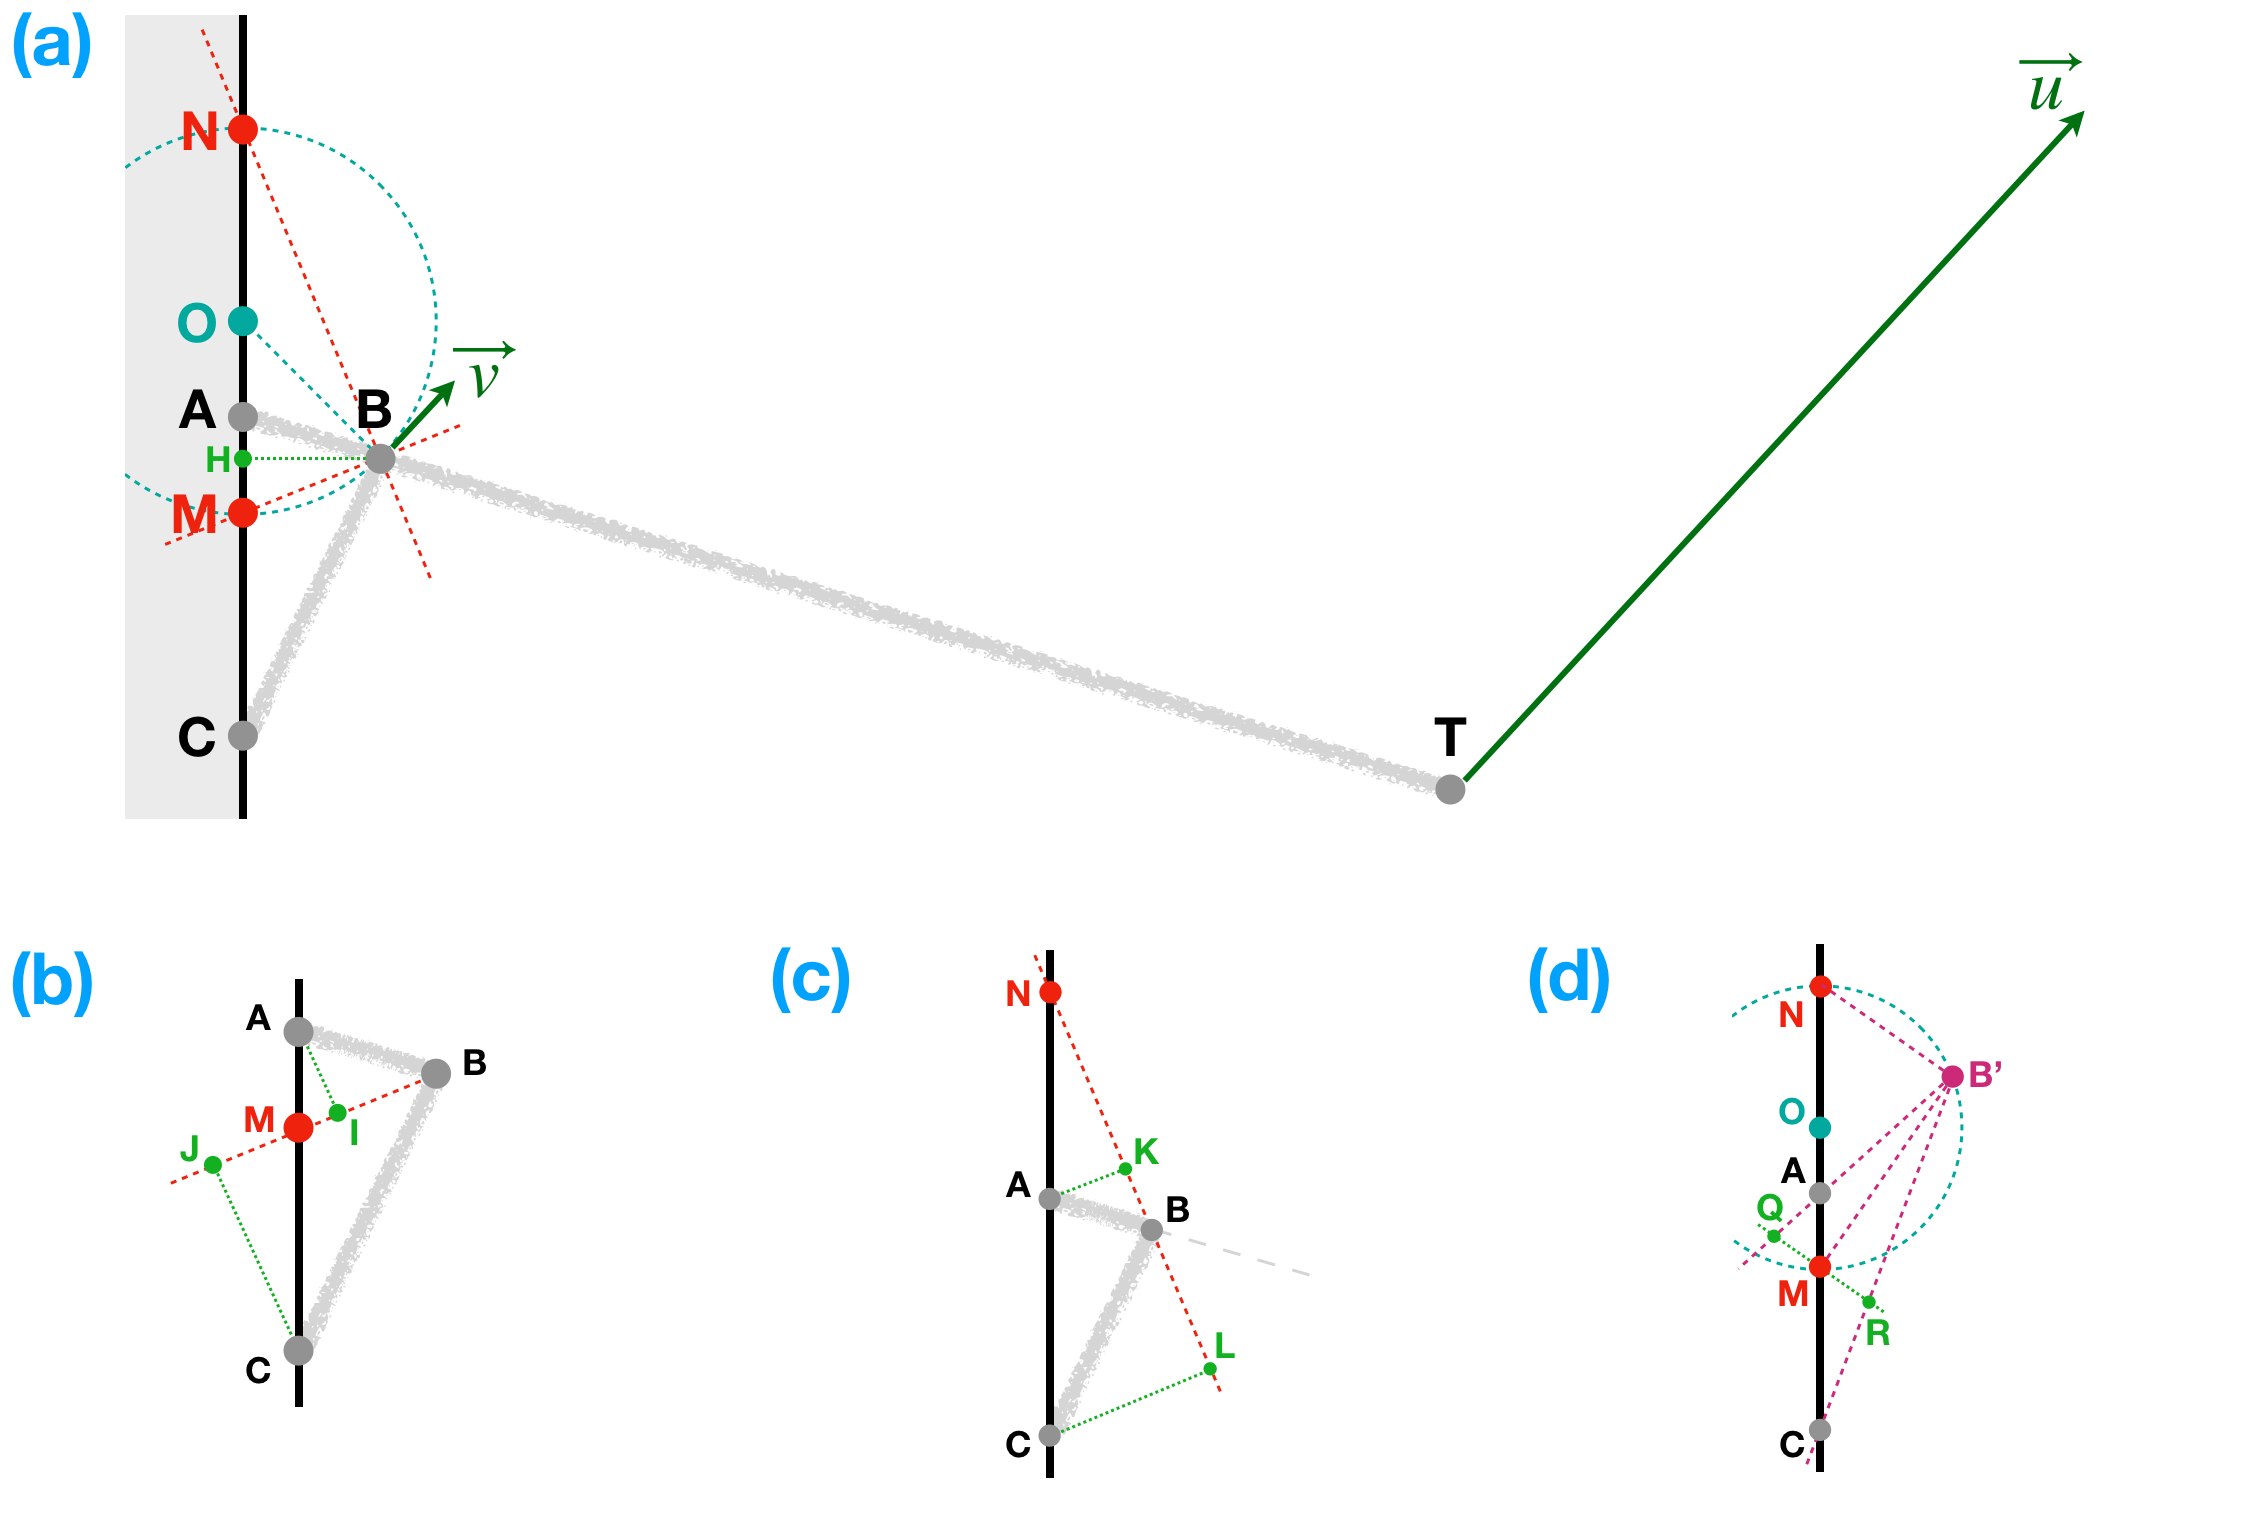
\includegraphics[width=\textwidth,keepaspectratio]{Problem_3/Figs/S3.png}
\end{center}

\ \

Kỳ thú và sảng khoái hơn nữa, với một điểm B' bất kỳ trên đường tròn tâm O đường kính MN thì ta luôn có B'M là phân giác góc $\widehat{\text{AB'C}}$. Chúng ta có thể chứng minh vắn như sau:

\begin{itemize}
     \item Từ M kẻ đường song song với B'N, cắt đường kéo dài B'A về phía A tại điểm Q và cắt đoạn B'C tại điểm R (xem hình minh họa \textbf{d}). Theo định lý Thalès, với MQ $\parallel$ B'N thì ta có $\overline{\text{MQ}}:\overline{\text{B'N}} = \overline{\text{AM}}:\overline{\text{AN}}$, với MR $\parallel$ B'N thì ta có $\overline{\text{MR}}:\overline{\text{B'N}} = \overline{\text{CM}}:\overline{\text{CN}}$. Sử dụng \eqref{distance}, thu được $\overline{\text{MQ}}=\overline{\text{QR}}$, tức M là trung điểm đoạn QR. Cùng với B'M vuông góc với QR, ta kết luận rằng tam giác $\Delta_\text{QB'R}$ cân ở B' và B'M là phân giác góc $\widehat{\text{QB'R}} \equiv \widehat{\text{AB'C}}$.
 \end{itemize}
    
\ \ 

Trong quá trình nở đều ra do nhiệt độ tăng lên (do thép là kim loại nở ra vì nhiệt), do tỉ số $\overline{\text{AB}}:\overline{\text{BC}}$ không đổi nên khớp B sẽ di chuyển trên đường tròn tâm O đường kính MN. Khoảng cách OB không đổi, tức véc-tơ vận tốc $\overrightarrow{v}$ của B sẽ vuông góc với đoạn OB. Như đã cho ở đề bài, thành phần vận tốc theo phương thẳng đứng của B là:
\begin{equation}
v_{\parallel} = \sin \widehat{\text{BOH}} .|\overrightarrow{v}| = \Big( \overline{\text{BH}}:\overline{\text{OB}}\Big) \vert \overrightarrow{v} \vert \ .
\label{v_veloc}
\end{equation}
Chiều cao $\overline{\text{BH}}$ có thể xác định được từ công thức Heron cho diện tích tam giác:
\begin{equation}
\begin{split}
\overline{\text{BH}} = \frac{2S(\Delta_{\text{ABC}})}{\overline{\text{AC}}} & = \frac{\sqrt{(s_1+s_2+s_3)(-s_1+s_2+s_3)(s_1-s_2+s_3)(s_1+s_2-s_3)}}{2s_3}
\\
& = \frac{\sqrt{(s_1^2+s_2^2+s_3^2)^2-2(s_1^4+s_2^4+s_3^4)}}{2s_3} \ .
\end{split}
\label{height}
\end{equation}
Chúng ta thế \eqref{radius} và \eqref{height} vào \eqref{v_veloc}, thu được giá trị độ lớn vận tốc của B:
\begin{equation}
\vert \overrightarrow{v} \vert = \frac{2s_1s_2 s_3^2}{(-s_1^2 + s_2^2)\sqrt{(s_1^2+s_2^2+s_3^2)^2-2(s_1^4+s_2^4+s_3^4)}} v_{\parallel} \ .
\label{v_mag}
\end{equation}
Thanh AT nở đều và quay quay khớp A ở vị trí cố định, nên do đồng dạng ta có liên hệ vận tốc:
 \begin{equation}
 \overrightarrow{u} = \left(\overline{\text{AT}} : \overline{\text{AB}} \right) . \overrightarrow{v} = \left( 1 + \frac{s_4}{s_1} \right) \overrightarrow{v} \ ,
 \end{equation}
 với $\overrightarrow{u}$ là vận tốc đầu thanh T. Thế nên, sử dụng \eqref{v_mag}:
\begin{equation}
\vert \overrightarrow{u} \vert = \frac{2s_1s_2 s_3^2 \left( 1 + \frac{s_4}{s_1}\right)}{(-s_1^2 + s_2^2)\sqrt{(s_1^2+s_2^2+s_3^2)^2-2(s_1^4+s_2^4+s_3^4)}} v_{\parallel} \ .
\label{u_mag}
\end{equation}
Vì $\overrightarrow{u} \parallel \overrightarrow{v}$ nên $\overrightarrow{u}$ cũng hợp với phương ngang góc $\theta = \widehat{\text{BOH}}$:
\begin{equation}
\begin{split}
 \theta &= \arcsin \Big( \overline{\text{BH}}:\overline{\text{OB}}\Big)
 \\
&= \arcsin \left[ \frac{(-s_1^2 + s_2^2)\sqrt{(s_1^2+s_2^2+s_3^2)^2-2(s_1^4+s_2^4+s_3^4)}}{2s_1s_2 s_3^2} \right] \ .
\end{split}
\label{angle}
\end{equation}

\ \ 

\textit{Dành cho các bạn muốn tìm hiểu sâu thêm, dễ dàng hơn để tổng quát với trường hợp hệ số nở về nhiệt của các thanh là khác nhau, nhưng cần phải phân tích vận tốc của khớp B ra thành phần quay và thành phần duỗi đối với từng thanh một. Phân tích này, thiết nghĩ, hơi vượt quá phạm vi kiến thức của học sinh THCS. Hy vọng sau khi đã vào cấp III, các bạn sẽ dành chút thời gian để tự giải lại bài tập theo hướng này.}